% !TEX root =  ../main.tex
\chapter{Étude d'un premier ordre par les 4 méthodes de discrétisation.}

\section{Introduction}
Durant la première séance de laboratoire, il nous a été demandé du calculer l'expression récurrente d'un premier ordre par les 4 méthodes de discrétisation, à savoir : 
\begin{itemize}
\item La méthode de Euler 1 ;
\item La méthode de Euler 2 ;
\item La méthode bilinéaire ;
\item La méthode équivalent échantillonné bloqué.
\end{itemize}
Une fois les 4 expressions calculées, l'objectif était d'utiliser le logiciel MATLAB afin de représenter les réponses temporelles et fréquentielles de ces 4 expressions. Ceci, dans la but d'analyser les différents paramètres de ces 4 méthodes de discrétisation.

\section{Rappels théoriques}

Actuellement, les méthodes de traitements numériques pour l'analyse des signaux ont largement pris le dessus comparé aux méthodes analogiques ancestrales. C'est pourquoi nous abordons les notions de procédés de discrétisation. En effet, en traitement numérique, un signal analogique est tout d'abord échantillonné (= discrétisé) avant d'être quantifié et finalement codé. La discrétisation est le procédé par lequel un signal continu est transformé un signal discret. Autrement dit, la discrétisation d'un signal continu f(t) revient à garder un certain nombre de valeurs discrètes (..., f(t0), f(t1), f(t2), ...) correspondant aux valeurs (..., t0, t1, t2, ...) de la variable t : On parle également d'échantillonnage pour les signaux. les différentes valeurs discrètes (..., f(t0), f(t1), f(t2), ...) varient en fonction de la période d'échantillonnage. La figure 1.1 ci-dessous présente le principe d'échantillonnage.
\begin{figure}[!ht]
\centering
	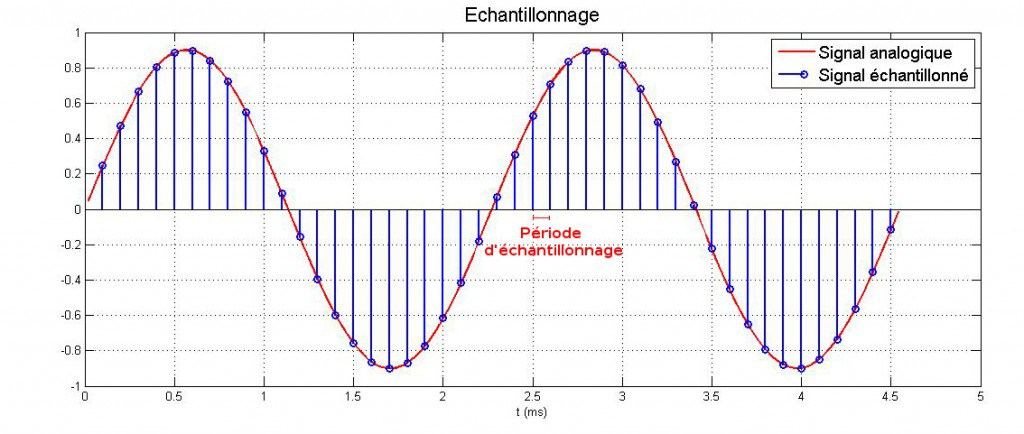
\includegraphics[scale=0.45]{images/echantillonnage.jpg}
	\caption{Échantillonnage d'un signal continu sinusoïdal.}
	\label{fig:échantillonnage}
\end{figure}

\newpage
Ayant introduit la notion de discrétisation, il est intéressant de rappeler le principe des 4 méthodes de discrétisation étudiées en laboratoire : 
\begin{description}
\item[La méthode de Euler 1] :  
\item[La méthode de Euler 2] : 
\item[La méthode bilinéaire] :  
\item[La méthode équivalent échantillonné bloqué] :  
\end{description}

\section{Analyse}


\section{Conclusion}

